\section{Simulation Verification}


\subsection{EKF Verification}
This section presents some simulation results that verify the EKF implementation on Odisseus

\subsubsection{Test 1}

In this test the following input data was used

\begin{equation}
R = 
\begin{pmatrix}
 1.0 & 0.0 \\
0.0 & 1.0 
\end{pmatrix}
\end{equation}

\begin{equation}
Q = 
\begin{pmatrix}
0.001 & 0.0 \\
0.0 & 0.001 
\end{pmatrix}
\end{equation}

The motion model $\mathbf{f}$ is according to equation \ref{odisseus_discrete} where the error vector $\mathbf{w}$ was set to zero.

The observation model function $\mathbf{h}$ was simply the identity function meaning returning the passed state vector

\begin{equation}
\mathbf{h}(\mathbf{x}, \mathbf{v}) = \mathbf{x}
\end{equation}

The error vector $\mathbf{v}$ was set to

\begin{equation}
\mathbf{v} = (0.0, 0.0)
\end{equation}

Finally, the following data was used

\begin{enumerate}
	\item $\Delta t = 0.5$
	\item $R = 2.5 cm$
	\item $v_L = v_R = 50 RPM$
	\item $L= 15 cm$ 
\end{enumerate}


\begin{figure}[!htb]
	\begin{center}
		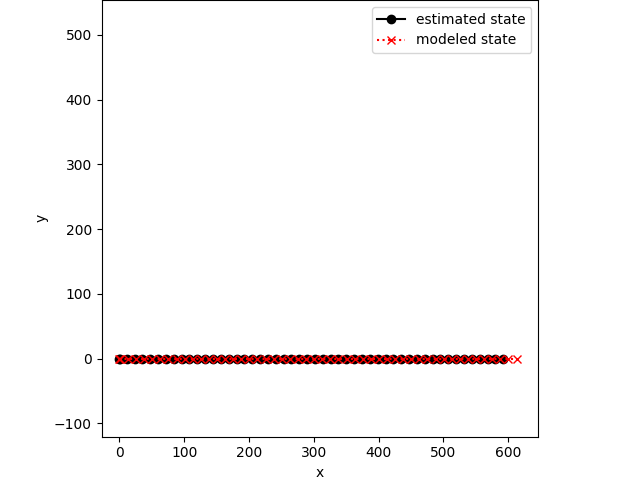
\includegraphics[scale=0.480]{imgs/ekf_straight_motion_1.png}
	\end{center}
	\caption{ Straight motion test 1.}
	\label{ekf_straight_motion_1}
\end{figure}

\begin{figure}[!htb]
	\begin{center}
		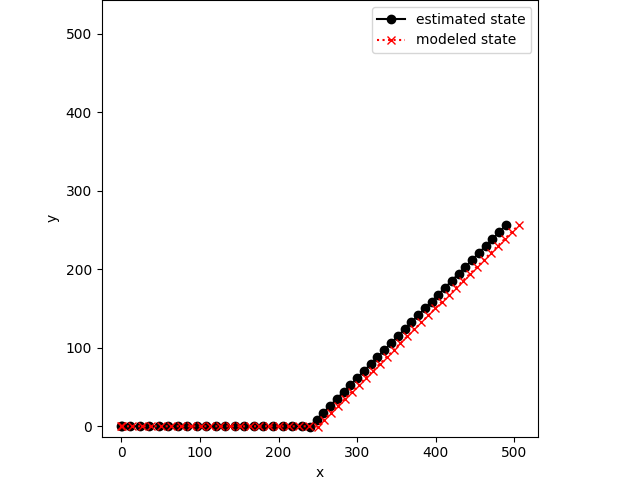
\includegraphics[scale=0.480]{imgs/ekf_change_direction_1.png}
	\end{center}
	\caption{ Change direction test 1.}
	\label{ekf_change_direction_1}
\end{figure}

\subsubsection{Test 2}

The second simulation test uses equation \ref{sonar_h} to model the sonar measurement

\begin{figure}[!htb]
	\begin{center}
		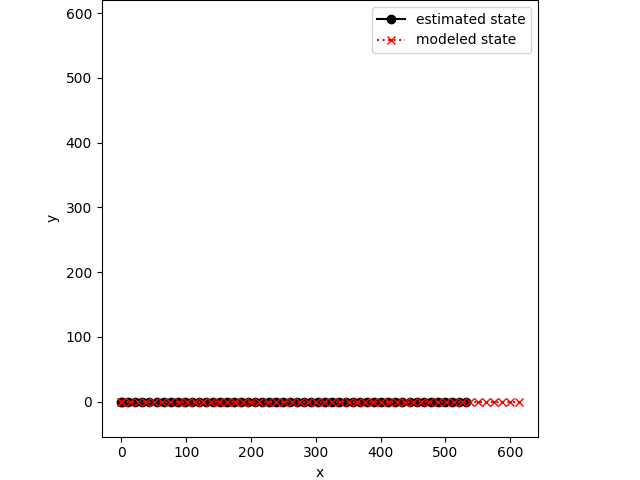
\includegraphics[scale=0.480]{imgs/ekf_straight_motion_2.png}
	\end{center}
	\caption{ Straight motion test 2.}
	\label{ekf_straight_motion_2}
\end{figure}
